\documentclass{article}

%change the margin of the paper
%\usepackage[legalpaper, margin=0.1in]{geometry}
%using the \substack
\usepackage{amsmath}
% \mathbbm{}
\usepackage{bbm}

% NOTE \pdv  partial differential equation
\usepackage{physics}

% hyperlink Here
\usepackage{hyperref}
\hypersetup{
    colorlinks=true,
    linkcolor=blue,
    filecolor=magenta,
    urlcolor=cyan,
}

% this is the package for block comment \begin{comment} and \end{comment}
\usepackage{verbatim}
\usepackage{imakeidx}
% For multiple rows in tabular environment.
\usepackage{multirow}
% use this package to strikeout the word /st{}
%the color package is for the \textcolor{red} to highlight the text
\usepackage{color,soul}
% to define newcolumntype and \arraybackslash
\usepackage{array}
% hyperref is to call /url. hyphen packege to avoid that the url is too long
\PassOptionsToPackage{hyphens}{url}\usepackage{hyperref}
%Todo list, \newlist \setlist...
\usepackage{enumitem,amssymb}
\newlist{todolist}{itemize}{2}
\setlist[todolist]{label=$\square$}

% for image inserting
\usepackage{graphicx}
\graphicspath{./Desktop/Homework/}
\usepackage{subfig}

% \iff \leqlsant
\usepackage{amssymb}



% Code block begin(lstlisting) and end(lstlisting)
\usepackage{listings}
\usepackage{color}

\definecolor{dkgreen}{rgb}{0,0.6,0}
\definecolor{gray}{rgb}{0.5,0.5,0.5}
\definecolor{mauve}{rgb}{0.58,0,0.82}


%NOTE: Change the "language" parameter here
\lstset{frame=tb,
  language=Matlab,
  aboveskip=3mm,
  belowskip=3mm,
  showstringspaces=false,
  columns=flexible,
  basicstyle={\small\ttfamily},
  numbers=none,
  numberstyle=\tiny\color{gray},
  keywordstyle=\color{blue},
  commentstyle=\color{dkgreen},
  stringstyle=\color{mauve},
  breaklines=true,
  breakatwhitespace=true,
  tabsize=3
}

% Macros
%%%%%%%%%%%% Text Color %%%%%%%%%%%%%%%
\definecolor{mypink1}{RGB}{219, 48, 233}
\definecolor{myred1}{RGB}{231, 76, 60}
\definecolor{myred2}{RGB}{203, 67, 53}
\definecolor{myblue1}{RGB}{52, 152, 219}
\definecolor{mygray}{gray}{0.6}

%% Table Style
\newcolumntype{C}{>{\center\arraybackslash}m{.70\columnwidth}}
\newcolumntype{Y}{>{\center\arraybackslash}m{2cm}}



%NOTE title Here
\title{Homework 8 Data Analysis}
\author{Hanyuan Zhu}



%%%%%%%%%%%%% NOTE Begin of Document %%%%%%%%%%%%%%%%%%%%%%%%%%%%%%%%%%%%%%%
%%%%%%%%%%%%%%%%%%%%%%%%%%%%%%%%%%%%%%%%%%%%%%%%%%%%%%%%%%%%%%%%%%%%%%%%%%%


\begin{document}

\maketitle
\subsection*{Question 1}
\paragraph{a.}

\begin{enumerate}
  \item Given N data points, $\{x_i | i = 1,2,...N\} $ and the distance frunction between Clusters , $ \Delta(C_i,C_j)$.
  \item $ C_{\Delta_t} = \{ C_i = \{x_i\} |  i = 1,...,N \}$ Initially each data point is a cluster, so we have a collection of clusters,
  \item  Iteratively, we merges two clusters with smallest distance, that is for $arg\min_{i,j} \Delta(C_i,C_j)$ then $ C_i \cup C_j = C_i $ .
\end{enumerate}

\paragraph{b.}

\begin{figure}[h]
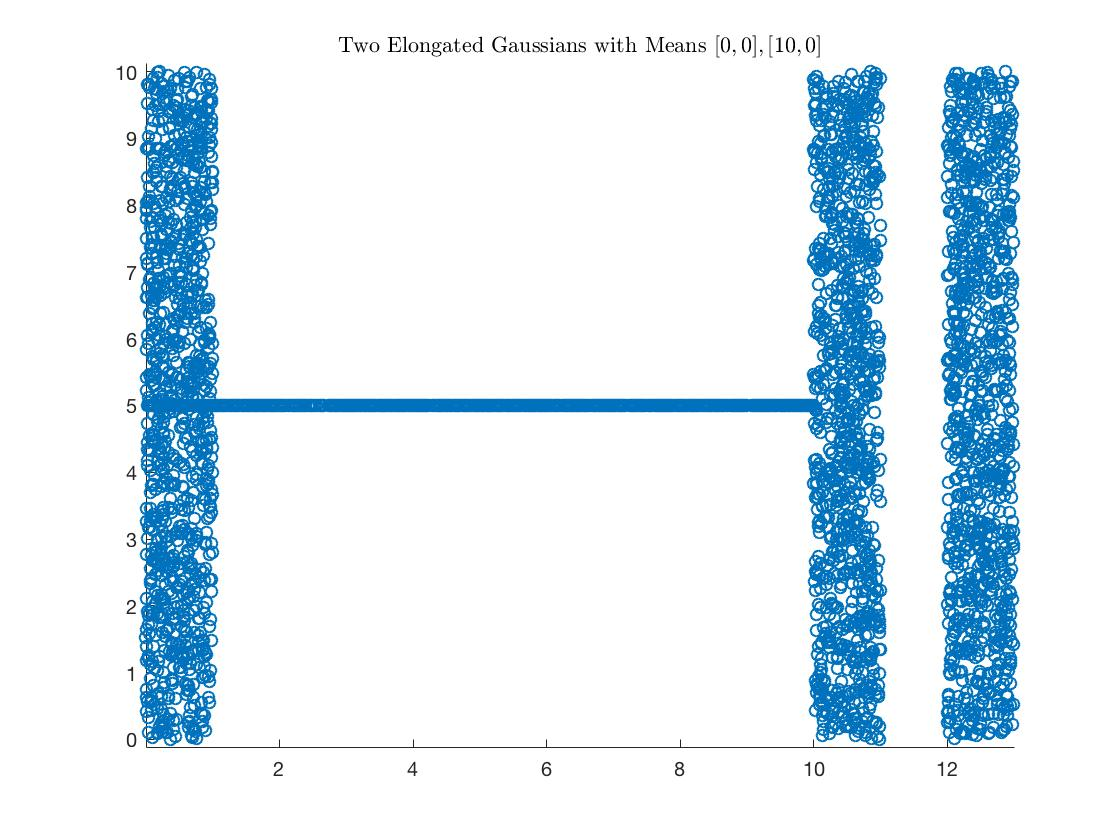
\includegraphics[width=8cm, height=8cm]{4a}
\end{figure}

Complete linkage clustering : it computes all pairwise distance between the elements in cluster 1 and the elements in cluster 2, and considers the largest value (i.e., maximum value) of these dissimilarities as the distance between the two clusters.
It tends to produce more compact clusters.

Single linkage clustering : It computes all pairwise dissimilarities between the elements in cluster 1 and the elements in cluster 2, and considers the smallest of these dissimilarities as a linkage criterion.
 It tends to produce long, “loose” clusters.

 \subsection*{Question 2}
\paragraph{a.}
$$ L_{sym}  = I  - D^{-\frac{1}{2}} W D^{-\frac{1}{2}}$$
D is degree matrix, and W is adjacent matrix of graph .
\paragraph{b.}
$$ L_{sym}  = D^{-\frac{1}{2}} L D^{-\frac{1}{2}}$$
Method 1: L has a eigenvalue $ \lambda = 0$ and the eigenvector is $ Lv=0 $ .
$$ L_{sym} D^{\frac{1}{2}} = D^{-\frac{1}{2}} L $$
$$ L_{sym} D^{\frac{1}{2}}v = D^{-\frac{1}{2}} Lv = 0$$
Therefore $ L_{sym} $ has eigenvalue 0 with eigenvector $D^{\frac{1}{2}}v$ .


\subsection*{Question 3}
\paragraph{a.}

Because of complete unweighted graph, the we have laplacian below,
$$ L_{rw}  = I  - D^{-1} W $$
where $D = \{d_i = n-1 | i = 1, 2, ... n\}$.

\begin{equation}
  (L_{rw})ij =
  \begin{cases}
    1, &i =j  \\
    \frac{1}{n-1}, &i \neq j
  \end{cases}
\end{equation}


\paragraph{b.}
It has eigenvalue $\frac{n}{n-1}$ with multiplicity n-1, and the last eigenvalue is 0.


\paragraph{c.}
By part b. we know such K =1 , which means 1 cluster.  Since a unweighted complete graph has no real cluster structure
inside it, every point is identical.

\subsection*{Question 4}

\paragraph{a.}
For traning part , to find the best parameter n for Knn.
\begin{itemize}
  \item 1. Compute the distance matrix for testting point respect to all training points.
  \item 2. For each point in test set, we choose the n nearest point and then to label it by the majority of labels among these n points.
  \item 3. Compupter the loss function by mislabelling. To minimize the loss function , we ge the optimized n.
\end{itemize}

To label incoming data
\begin{enumerate}
  \item Compute the distance matrix for incoming point respect to all labelled points.
  \item We choose the n nearest point and then to label it by the majority of labels among these n points.
\end{enumerate}

\paragraph{b.}
It wont be a useful result, because all test points will have same label, which is the majority from train set.

\subsection*{Question 5}

For unsupervise learning part, we can just use DBSCAN, because data intuitively are separated densely in 3 clusters. We just need to choose minPts and $\delta$ properly.
Let $\delta$ be sufficiently large but should be smaller than the gap between those intuitive clusters.

$y_i^{(s)}$ is the lebel of each point $x_i \in C^{(s)}$ from , and $l_i$ is the true Label

We have loss function $ loss = \frac{1}{n} \sum^{n}_{i=1} |y_i^{(s)} -l_i|  $

\end{document}
